\chapter{Forundersøgelse}

\section{GSM (JSA)}
\begin{table}[H] \centering
	\label{tab:GSM1}
\begin{tabular}{|p{6cm}|p{8cm}|}
	\hline
		\textbf{Løsning}				&GSM-modul \\ \hline
		\textbf{Producent} 			&Cinterion \\ \hline
		\textbf{Interface} 			&I2C, SPI, USB \\ \hline
		\textbf{Beskrivelse} 		&Hardware modul der kan tilkobles CSS-hovedenhed via SPI \\ \hline
		\textbf{Krav} 				&SIM kort og indgående programmerings kendskab \\ \hline
		\textbf{Fordele}				&Mest pålidelige løsning og ingen forsinkelse på SMS'er \\ \hline
		\textbf{Ulemper} 			&Kræver viden inden for Java eller Microsoft Windows Mobile programmering \\ \hline
		\textbf{Pris} 				&563,23 - 656,34 + SMS-takst \\ \hline
		\textbf{Link} 				&http://dk.farnell.com/cinterion/mc75i/module-gsm-gprs-edge-quad-band/dp/1718875 \newline
									 http://dk.farnell.com/cinterion/tc65i/mod-gsm-gprs-quad-band-tcp-ip/dp/1718877 \\ \hline
		\multicolumn{2}{|c|}{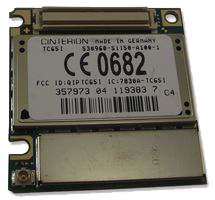
\includegraphics[height=3cm]{billeder/GSM_TC65I}} 	
\\ \hline

\end{tabular}
\end{table}

\begin{table}[H] \centering
	\label{tab:GSM2}
\begin{tabular}{|p{6cm}|p{8cm}|}
	\hline
		\textbf{Løsning}				&API \\ \hline
		\textbf{Producent} 			&Clickatell \\ \hline
		\textbf{Interface} 			&HTTP, HTTPS, FTP, SMPP, XML, SOAP, SMTP, COM obj.\\ \hline
		\textbf{Beskrivelse} 		&Software baseret API modul \\ \hline
		\textbf{Krav} 				&Forbindelse til internettet \\ \hline
		\textbf{Fordele}				&Let at programmere \\ \hline
		\textbf{Ulemper} 			&Kræver forbindelse til internettet \\ \hline
		\textbf{Pris} 				&0,762 kr. pr. SMS \\ \hline
		\textbf{Link} 				&https://www.clickatell.com/apis-scripts/ \\ \hline	
		\multicolumn{2}{|c|}{
			
\includegraphics[height=3cm]{billeder/GSM_Clickatell}} \\ \hline	
\end{tabular}
\end{table}

\begin{table}[H] \centering
	\label{tab:GSM3}
\begin{tabular}{|p{6cm}|p{8cm}|}
	\hline
		\textbf{Løsning}				&Arduino + GSM shield \\ \hline
		\textbf{Producent} 			&Arduino \\ \hline
		\textbf{Interface} 			&Internt \\ \hline
		\textbf{Beskrivelse} 		&Single-board computer med GSM modul\\ \hline
		\textbf{Krav} 				&SIM kort \\ \hline
		\textbf{Fordele}				&Let at programmere \\ \hline
		\textbf{Ulemper} 			&\\ \hline
		\textbf{Pris} 				&149,- + 515,- + SMS takst\\ \hline
		\textbf{Link} 				&http://arduino.cc/ \\ \hline		
		\multicolumn{2}{|c|}{
			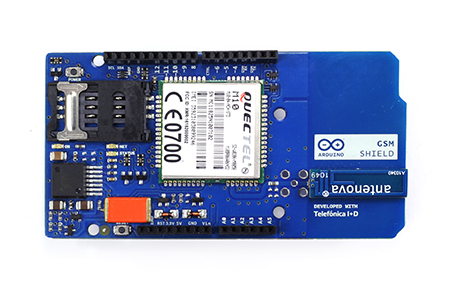
\includegraphics[height=3cm]{billeder/GSM_Arduino}} \\ \hline	
\end{tabular}
\end{table}
\subsection{GSM-valg}
Vi har valgt at bruge Clickatell-løsningen, da den er let at implementere og fleksibel og billig i opstartsomkostninger.

\newpage
\section{Lås (PO)}
\input{filer/forundersoegelse/laas}
\subsection{Låsvalg}
Valget et faldet på den elektromagnetiske lås fra KingGo. Denne lås er valgt da den er simpel og let at sætte op, og da der ikke skal fræses ud for at benytte denne type lås. Ydermere så vil låsen automatisk låse sig fast, hvis modtager pladen er ude for rækkevidde og denne fysisk skubbes hen til elektromagneten.

\newpage
\section{Babyalarm (JC)}
\begin{table}[!h] \centering	
	\label{tab:laas1}
\begin{tabular}{|p{6cm}|p{8cm}|}
	\hline
		\textbf{Navn}				&Philips SCD505 \\ \hline
		\textbf{Rækkevidde} 			&330 \\ \hline
		\textbf{Lyd:} 		&Justerbar lydniveau. 
							Lys i forældreenheden angiver lydniveau ved babyen \\ \hline
		\textbf{Batteri} 		&Delvist genopladelig \\ \hline
		\textbf{Stråling} 				&Høj \\ \hline
		\textbf{Pris} 				&549 kr \\ \hline
		\textbf{Link} 				&http://goo.gl/pw06P9 \\ \hline	
		\multicolumn{2}{|c|}{
			\raisebox{-0.91\height}{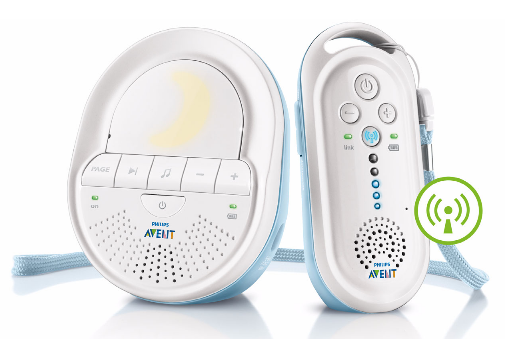
\includegraphics[height=3cm]{billeder/SCD505}}} \\ \hline	
\end{tabular}
\end{table}

\begin{table}[!htbp] \centering
	\label{tab:laas2}
\begin{tabular}{|p{6cm}|p{8cm}|}
	\hline
		\textbf{Navn}				&Supernova D7 \\ \hline
		\textbf{Rækkevidde} 			&600m \\ \hline
		\textbf{Lyd} 		&Ukendt\\ \hline
		\textbf{Batteri} 		&2 genopladelige batterier \\ \hline
		\textbf{Pris} 				&999 kr \\ \hline
		\textbf{Stråling} 				&Lav \\ \hline
		\textbf{Link} 				&http://goo.gl/JFZcf5\\ \hline	
		\multicolumn{2}{|c|}{
			\raisebox{-0.91\height}{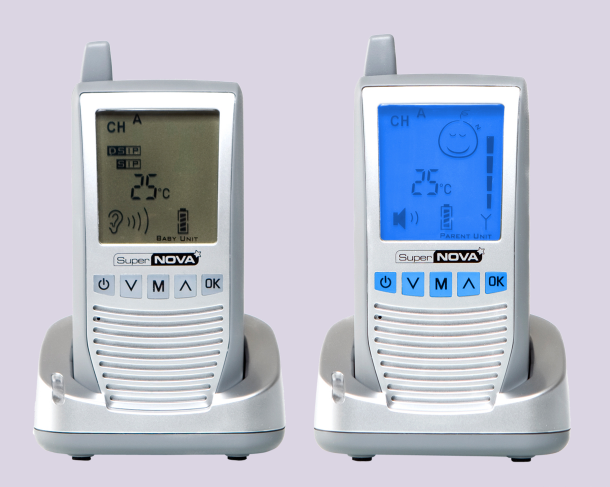
\includegraphics[height=2.8cm]{billeder/Supernova}}} \\ \hline	
\end{tabular}
\end{table}
\subsection{Babyalarm sammenligning}
Vi har valgt at lave en forundersøgelse på babyalarmer for at få en indikation af hvad markedet tilbyder, imod det vi kommer til at tilbyde med vores babyalarm.

Vi har valgt at vores babyalarm skal reagere på lydniveauer højere end 40 dB. Da vores babyalarm ikke bliver trådløs så undgår vi ting som stråling og batteri tid. Vores rækkevidde bliver dog betydeligt mindre end den typiske babyalarm, igen på grund af at den ikke er trådløs. Vores babyalarm er tænkt som en stationær enhed som kan placeres i et barneværelse og altså ikke som en transportabel babyalarm som man typisk ser.

